\section{General Introduction to Feynman Diagram in Many-body Problem}
\subsection{A Brief Intro to Quasi-particle}
\redp{Quasi particles arise from the fact that when a real particle moves through the system, it pushes or pulls on its neighbours and thus becomes surrounded by a \textbf{'cloud' of agitated particles}.}

The particle cloud "shields" or "screens" the real particles so that quasi particles interact only weakly with one another. The presence of the cloud also makes the properties of the quasi particle different from that of the real particle-it may have an "\textbf{effective mass}" different from the real mass, and a "\textbf{lifetime}". These properties of quasi particles are directly observable experimentally. It should be remarked that \redp{the quasi particle is in an excited energy level of the many-body system}. Hence it is referred to as an '\textbf{elementary excitation}' of the system. We now consider some examples of quasi particles.
\begin{easylist}
\NewList

@ Quasi ion in a classical liquid
\begin{figure}[H]
    \centering
\tikzset{every picture/.style={line width=0.75pt}} %set default line width to 0.75pt        

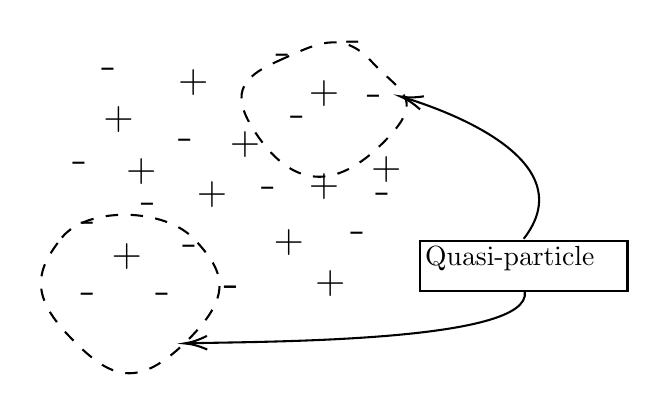
\begin{tikzpicture}[x=0.75pt,y=0.75pt,yscale=-1,xscale=1]
%uncomment if require: \path (0,300); %set diagram left start at 0, and has height of 300

%Shape: Polygon Curved [id:ds393267198766974] 
\draw  [dash pattern={on 4.5pt off 4.5pt}] (104.52,151.27) .. controls (116.52,136.27) and (154.03,136.65) .. (168.52,152.27) .. controls (183,167.88) and (187.52,179.27) .. (163.52,202.27) .. controls (139.52,225.27) and (126.52,218.27) .. (107.52,198.27) .. controls (88.52,178.27) and (92.52,166.27) .. (104.52,151.27) -- cycle ;
%Shape: Polygon Curved [id:ds5938648082047331] 
\draw  [dash pattern={on 4.5pt off 4.5pt}] (208.52,66.27) .. controls (226.52,58.27) and (239.03,50.65) .. (253.52,66.27) .. controls (268,81.88) and (281.52,84.27) .. (257.52,107.27) .. controls (233.52,130.27) and (214.52,124.27) .. (199.52,103.27) .. controls (184.52,82.27) and (190.52,74.27) .. (208.52,66.27) -- cycle ;
%Curve Lines [id:da7350178540870457] 
\draw    (327,151.88) .. controls (354.95,116) and (296.92,92.23) .. (269.18,83.77) ;
\draw [shift={(267.52,83.27)}, rotate = 376.5] [color={rgb, 255:red, 0; green, 0; blue, 0 }  ][line width=0.75]    (10.93,-3.29) .. controls (6.95,-1.4) and (3.31,-0.3) .. (0,0) .. controls (3.31,0.3) and (6.95,1.4) .. (10.93,3.29)   ;
%Curve Lines [id:da8754807282204362] 
\draw    (327.52,177.27) .. controls (331.46,201.89) and (200.54,201.29) .. (165.07,202.22) ;
\draw [shift={(163.52,202.27)}, rotate = 358.26] [color={rgb, 255:red, 0; green, 0; blue, 0 }  ][line width=0.75]    (10.93,-3.29) .. controls (6.95,-1.4) and (3.31,-0.3) .. (0,0) .. controls (3.31,0.3) and (6.95,1.4) .. (10.93,3.29)   ;

% Text Node
\draw (127,152.88) node [anchor=north west][inner sep=0.75pt]  [font=\Large] [align=left] {+};
% Text Node
\draw (141,128.88) node [anchor=north west][inner sep=0.75pt]  [font=\LARGE] [align=left] {\mbox{-}};
% Text Node
\draw (161,148.88) node [anchor=north west][inner sep=0.75pt]  [font=\LARGE] [align=left] {\mbox{-}};
% Text Node
\draw (148,171.88) node [anchor=north west][inner sep=0.75pt]  [font=\LARGE] [align=left] {\mbox{-}};
% Text Node
\draw (112,171.88) node [anchor=north west][inner sep=0.75pt]  [font=\LARGE] [align=left] {\mbox{-}};
% Text Node
\draw (112,137.88) node [anchor=north west][inner sep=0.75pt]  [font=\LARGE] [align=left] {\mbox{-}};
% Text Node
\draw (168,122.88) node [anchor=north west][inner sep=0.75pt]  [font=\Large] [align=left] {+};
% Text Node
\draw (205,145.88) node [anchor=north west][inner sep=0.75pt]  [font=\Large] [align=left] {+};
% Text Node
\draw (181,168.88) node [anchor=north west][inner sep=0.75pt]  [font=\LARGE] [align=left] {\mbox{-}};
% Text Node
\draw (181,168.88) node [anchor=north west][inner sep=0.75pt]  [font=\LARGE] [align=left] {\mbox{-}};
% Text Node
\draw (242,142.88) node [anchor=north west][inner sep=0.75pt]  [font=\LARGE] [align=left] {\mbox{-}};
% Text Node
\draw (199,120.88) node [anchor=north west][inner sep=0.75pt]  [font=\LARGE] [align=left] {\mbox{-}};
% Text Node
\draw (222,118.88) node [anchor=north west][inner sep=0.75pt]  [font=\Large] [align=left] {+};
% Text Node
\draw (184,98.88) node [anchor=north west][inner sep=0.75pt]  [font=\Large] [align=left] {+};
% Text Node
\draw (159,97.88) node [anchor=north west][inner sep=0.75pt]  [font=\LARGE] [align=left] {\mbox{-}};
% Text Node
\draw (254,123.88) node [anchor=north west][inner sep=0.75pt]  [font=\LARGE] [align=left] {\mbox{-}};
% Text Node
\draw (213,86.88) node [anchor=north west][inner sep=0.75pt]  [font=\LARGE] [align=left] {\mbox{-}};
% Text Node
\draw (250,76.88) node [anchor=north west][inner sep=0.75pt]  [font=\LARGE] [align=left] {\mbox{-}};
% Text Node
\draw (206,56.88) node [anchor=north west][inner sep=0.75pt]  [font=\LARGE] [align=left] {\mbox{-}};
% Text Node
\draw (240,50.88) node [anchor=north west][inner sep=0.75pt]  [font=\LARGE] [align=left] {\mbox{-}};
% Text Node
\draw (252,110.88) node [anchor=north west][inner sep=0.75pt]  [font=\Large] [align=left] {+};
% Text Node
\draw (222,73.88) node [anchor=north west][inner sep=0.75pt]  [font=\Large] [align=left] {+};
% Text Node
\draw (225,165.88) node [anchor=north west][inner sep=0.75pt]  [font=\Large] [align=left] {+};
% Text Node
\draw (159,68.88) node [anchor=north west][inner sep=0.75pt]  [font=\Large] [align=left] {+};
% Text Node
\draw (123,86.88) node [anchor=north west][inner sep=0.75pt]  [font=\Large] [align=left] {+};
% Text Node
\draw (108,108.88) node [anchor=north west][inner sep=0.75pt]  [font=\LARGE] [align=left] {\mbox{-}};
% Text Node
\draw (122,63.88) node [anchor=north west][inner sep=0.75pt]  [font=\LARGE] [align=left] {\mbox{-}};
% Text Node
\draw (134,111.88) node [anchor=north west][inner sep=0.75pt]  [font=\Large] [align=left] {+};
% Text Node
\draw    (277,152.88) -- (377,152.88) -- (377,176.88) -- (277,176.88) -- cycle  ;
\draw (278,153.88) node [anchor=north west][inner sep=0.75pt]   [align=left] {Quasi-particle};


\end{tikzpicture}

    \caption{Quasi particles in a Liquid of Positive and Negative Ions}
    \label{fig:quasi-particle-example}
\end{figure}
From Fig.\ref{fig:quasi-particle-example}, we know, from more powerful terminology of QFT:
\begin{center}
    "bare" particle + "clothing"/"cloud" = "dressed"/"renormalized" particle
\end{center}
For example, in quantum electrodynamics a 'bare' electron interacting with a field of photons acquires a cloud of virtual photons around it, converting it into the 'dressed' electron. In a similar manner, the interaction between real particles is called the 'bare' interaction, while the weak interaction between quasi particles is referred to as the 'effective' or "dressed" or "renormalized" interaction. \bluep{It should be noted that each bare particle is simultaneously the 'core' of a quasi particle and a transient 'member' of the cloud of several other quasi particles.}

The free quasi particles have a new energy law as 
$$\epsilon^{\prime}=\frac{p^{2}}{2 m^{*}} \quad \text { instead of } \quad \epsilon=\frac{p^{2}}{2 m}$$
where $m^*$ is the effective mass. The difference 
$$\epsilon_{quasi}-\epsilon_{bare}=\epsilon_{self}$$
is called \redp{\textbf{"self-energy"}} of the quasi particle.

@ Quantum System: quasi electreon in electron gas

The ' electron gas' is a simple model often used to describe many-body effects in metals. It consists of a box containing a large number of electrons interacting by means of the Coulomb force. In addition, there is a uniform, fixed, positive charge 'background' put into the box in order to keep the whole system electrically neutral. In the ground state, the electrons are spread out uniformly in the box.

Suppose now that we have a single, well-localized electron which we shoot into the electron gas  Because of the repulsive Coulomb interaction
between electrons, this extra electron repels other electrons away from it, so we get an empty space near the extra electron, and repelled electrons further away(Fig.\ref{fig:quasi-particle-example2}). This empty region may be viewed in a more detailed or microscopic way as composed of \redp{'holes'} in the electron gas. That is, the extra electron has "lifted out" electrons from the uniform charge distribution in its vicinity, thus creating 'holes' in this charge distribution, and has 'put down' these lifted-out electrons further away.
\begin{figure}[H]
    \centering
\tikzset {_0o14ioo3g/.code = {\pgfsetadditionalshadetransform{ \pgftransformshift{\pgfpoint{0 bp } { 0 bp }  }  \pgftransformscale{1 }  }}}
\pgfdeclareradialshading{_73ww2zakf}{\pgfpoint{0bp}{0bp}}{rgb(0bp)=(1,1,1);
rgb(12.019342694963727bp)=(1,1,1);
rgb(25bp)=(0,0,0);
rgb(400bp)=(0,0,0)}
\tikzset{_98ggw9slw/.code = {\pgfsetadditionalshadetransform{\pgftransformshift{\pgfpoint{0 bp } { 0 bp }  }  \pgftransformscale{1 } }}}
\pgfdeclareradialshading{_52d0oeat9} { \pgfpoint{0bp} {0bp}} {color(0bp)=(transparent!0);
color(12.019342694963727bp)=(transparent!0);
color(25bp)=(transparent!10);
color(400bp)=(transparent!10)} 
\pgfdeclarefading{_yzsmf2mqd}{\tikz \fill[shading=_52d0oeat9,_98ggw9slw] (0,0) rectangle (50bp,50bp); } 
\tikzset{every picture/.style={line width=0.75pt}} %set default line width to 0.75pt        

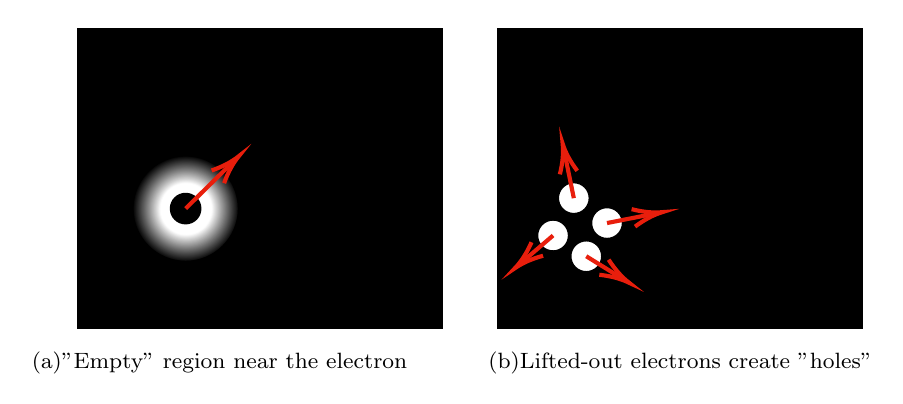
\begin{tikzpicture}[x=0.75pt,y=0.75pt,yscale=-1,xscale=1]
%uncomment if require: \path (0,300); %set diagram left start at 0, and has height of 300

%Shape: Rectangle [id:dp842398765103643] 
\draw  [fill={rgb, 255:red, 0; green, 0; blue, 0 }  ,fill opacity=1 ] (59.93,58.88) -- (235.32,58.88) -- (235.32,203.27) -- (59.93,203.27) -- cycle ;
%Shape: Circle [id:dp5878809314291961] 
\path  [shading=_73ww2zakf,_0o14ioo3g,path fading= _yzsmf2mqd ,fading transform={xshift=2}] (85.93,145.54) .. controls (85.93,131.37) and (97.42,119.88) .. (111.59,119.88) .. controls (125.76,119.88) and (137.25,131.37) .. (137.25,145.54) .. controls (137.25,159.71) and (125.76,171.2) .. (111.59,171.2) .. controls (97.42,171.2) and (85.93,159.71) .. (85.93,145.54) -- cycle ; % for fading 
 \draw   (85.93,145.54) .. controls (85.93,131.37) and (97.42,119.88) .. (111.59,119.88) .. controls (125.76,119.88) and (137.25,131.37) .. (137.25,145.54) .. controls (137.25,159.71) and (125.76,171.2) .. (111.59,171.2) .. controls (97.42,171.2) and (85.93,159.71) .. (85.93,145.54) -- cycle ; % for border 

%Shape: Circle [id:dp649192880176533] 
\draw  [fill={rgb, 255:red, 0; green, 0; blue, 0 }  ,fill opacity=1 ] (104.47,145.54) .. controls (104.47,141.61) and (107.66,138.42) .. (111.59,138.42) .. controls (115.53,138.42) and (118.72,141.61) .. (118.72,145.54) .. controls (118.72,149.48) and (115.53,152.67) .. (111.59,152.67) .. controls (107.66,152.67) and (104.47,149.48) .. (104.47,145.54) -- cycle ;
%Straight Lines [id:da47546531201986364] 
\draw [color={rgb, 255:red, 232; green, 30; blue, 12 }  ,draw opacity=1 ][line width=1.5]    (111.59,145.54) -- (135.11,122.37) ;
\draw [shift={(137.25,120.27)}, rotate = 495.43] [color={rgb, 255:red, 232; green, 30; blue, 12 }  ,draw opacity=1 ][line width=1.5]    (14.21,-4.28) .. controls (9.04,-1.82) and (4.3,-0.39) .. (0,0) .. controls (4.3,0.39) and (9.04,1.82) .. (14.21,4.28)   ;
%Shape: Rectangle [id:dp08609024153608191] 
\draw  [fill={rgb, 255:red, 0; green, 0; blue, 0 }  ,fill opacity=1 ] (261.93,58.88) -- (437.32,58.88) -- (437.32,203.27) -- (261.93,203.27) -- cycle ;
%Shape: Circle [id:dp8820237303823028] 
\draw  [fill={rgb, 255:red, 255; green, 255; blue, 255 }  ,fill opacity=1 ] (291,140.51) .. controls (291,136.3) and (294.41,132.88) .. (298.63,132.88) .. controls (302.84,132.88) and (306.25,136.3) .. (306.25,140.51) .. controls (306.25,144.72) and (302.84,148.13) .. (298.63,148.13) .. controls (294.41,148.13) and (291,144.72) .. (291,140.51) -- cycle ;
%Shape: Circle [id:dp5770389827427272] 
\draw  [fill={rgb, 255:red, 255; green, 255; blue, 255 }  ,fill opacity=1 ] (307,152.51) .. controls (307,148.3) and (310.41,144.88) .. (314.63,144.88) .. controls (318.84,144.88) and (322.25,148.3) .. (322.25,152.51) .. controls (322.25,156.72) and (318.84,160.13) .. (314.63,160.13) .. controls (310.41,160.13) and (307,156.72) .. (307,152.51) -- cycle ;
%Shape: Circle [id:dp025362450260817182] 
\draw  [fill={rgb, 255:red, 255; green, 255; blue, 255 }  ,fill opacity=1 ] (297,168.51) .. controls (297,164.3) and (300.41,160.88) .. (304.63,160.88) .. controls (308.84,160.88) and (312.25,164.3) .. (312.25,168.51) .. controls (312.25,172.72) and (308.84,176.13) .. (304.63,176.13) .. controls (300.41,176.13) and (297,172.72) .. (297,168.51) -- cycle ;
%Shape: Circle [id:dp9389847020012084] 
\draw  [fill={rgb, 255:red, 255; green, 255; blue, 255 }  ,fill opacity=1 ] (281,158.51) .. controls (281,154.3) and (284.41,150.88) .. (288.63,150.88) .. controls (292.84,150.88) and (296.25,154.3) .. (296.25,158.51) .. controls (296.25,162.72) and (292.84,166.13) .. (288.63,166.13) .. controls (284.41,166.13) and (281,162.72) .. (281,158.51) -- cycle ;
%Straight Lines [id:da4209538731972077] 
\draw [color={rgb, 255:red, 232; green, 30; blue, 12 }  ,draw opacity=1 ][line width=1.5]    (298.63,140.51) -- (293.85,117.21) ;
\draw [shift={(293.25,114.27)}, rotate = 438.42] [color={rgb, 255:red, 232; green, 30; blue, 12 }  ,draw opacity=1 ][line width=1.5]    (14.21,-4.28) .. controls (9.04,-1.82) and (4.3,-0.39) .. (0,0) .. controls (4.3,0.39) and (9.04,1.82) .. (14.21,4.28)   ;
%Straight Lines [id:da6368743975733171] 
\draw [color={rgb, 255:red, 232; green, 30; blue, 12 }  ,draw opacity=1 ][line width=1.5]    (314.63,152.51) -- (338.31,147.85) ;
\draw [shift={(341.25,147.27)}, rotate = 528.86] [color={rgb, 255:red, 232; green, 30; blue, 12 }  ,draw opacity=1 ][line width=1.5]    (14.21,-4.28) .. controls (9.04,-1.82) and (4.3,-0.39) .. (0,0) .. controls (4.3,0.39) and (9.04,1.82) .. (14.21,4.28)   ;
%Straight Lines [id:da3789740110796589] 
\draw [color={rgb, 255:red, 232; green, 30; blue, 12 }  ,draw opacity=1 ][line width=1.5]    (304.63,168.51) -- (322.7,179.69) ;
\draw [shift={(325.25,181.27)}, rotate = 211.74] [color={rgb, 255:red, 232; green, 30; blue, 12 }  ,draw opacity=1 ][line width=1.5]    (14.21,-4.28) .. controls (9.04,-1.82) and (4.3,-0.39) .. (0,0) .. controls (4.3,0.39) and (9.04,1.82) .. (14.21,4.28)   ;
%Straight Lines [id:da1630717526737726] 
\draw [color={rgb, 255:red, 232; green, 30; blue, 12 }  ,draw opacity=1 ][line width=1.5]    (288.63,158.51) -- (272.53,172.31) ;
\draw [shift={(270.25,174.27)}, rotate = 319.38] [color={rgb, 255:red, 232; green, 30; blue, 12 }  ,draw opacity=1 ][line width=1.5]    (14.21,-4.28) .. controls (9.04,-1.82) and (4.3,-0.39) .. (0,0) .. controls (4.3,0.39) and (9.04,1.82) .. (14.21,4.28)   ;

% Text Node
\draw (256,212.88) node [anchor=north west][inner sep=0.75pt]  [font=\footnotesize] [align=left] {(b)Lifted-out electrons create "holes"};
% Text Node
\draw (36,212.88) node [anchor=north west][inner sep=0.75pt]  [font=\footnotesize] [align=left] {(a)"Empty" region near the electron};


\end{tikzpicture}
    \caption{Extra Electron Pushes Other Electrons Away}
    \label{fig:quasi-particle-example2}
\end{figure}

@ Bogoliubov quasi particles ("bogolons")

These are the elementary excitations in a superconductor. We include them here since they are called quasi particles, but actually their structure is quite different from the 'particle plus cloud' picture described above. They consist of a linear combination ofan electron in state $(+k, \uparrow)$ and a hole $^{\prime}$ in $(-k, \downarrow)$.

\end{easylist}

\subsection{A Brief Intro to Collective Excitations}
As we have seen, the quasi particle consists of the original real, individual particle, plus a cloud of disturbed neighbours. It behaves very much like an
individual particle, except that it has an effective mass and a lifetime. But there also exist other kinds of fictitious particles in many-body systems, i.e., 'collective excitations'. These do not centre around individual particles, but instead involve collective, wavelike motion of all the particles in the system
simultaneously. Here are some examples:
\begin{easylist}
\NewList
@ Plasmons

If a thin metal foil is bombarded with high energy electrons, it is possible to set up sinusoidal oscillations in the density of the electron gas in the foil. This is known as a \bluep{'plasma wave'}, and it has a frequency $\omega_p$ and wavelength $\lambda_p$. \bluep{The plasma wave may be visualized as built up of 'holes' in the low-density regions and extra electrons in the high-density regions}. Just as light waves are quantized into units having energy $E=\hbar \omega$ called photons, plasma waves are quantized into units with energy $E_{p}=\hbar \omega_{p}$ called plasmons.

@ phonons

Sound waves are sinusoidal oscillations in the crystal lattice ofa solid. They are quantized into collective excitations called 'phonons'.

@ Magnons

In ferromagnets there are regular fluctuations in the density of spin angular momentum known as spin waves. The collective excitation here is the spin
wave quantum known as the 'magnon".
\end{easylist}

\subsection{Propagators-the Keys to the Many-body Problem}
The idea behind the propagator method is this: the detailed description of a many-body system requires in the classical case the position of each particle as a function of time, or in the quantum case, the time dependent wave function of the whole system. Fortunately, it turns out that \textbf{in order to find the important physical properties of a system it is not necessary to know the detailed behaviour of each particle in the system, but rather just the average behaviour of one or two typical particles.} \bluep{The quantities which describe this average behaviour are the\textit{ one-particle propagator} and \textit{two-particle propagator} respectively, and physical properties may be calculated directly from them.}

\begin{imp}
\textbf{One-particle propagator}: we put a particle into the interacting system at point $r_{1}$ at time $t_{1}$ and let it move through the system colliding with the other particles for a while (i.e., let it "propagate" through the system). Then the one-particle propagator is the probability (or in quantum systems, the probability amplitude) that the particle will be observed at the point $r_{2}$ at time $t_{2} .$ (Note that instead of putting the particle in at a definite point, it is sometimes more convenient to put it in with definite momentum, say $p_{1},$ and observe it later with momentum $p_{2} .$ ) \bluep{The single-particle propagator yields directly the energies and lifetimes of quasi particles. It also gives the momentum distribution, spin and particle density and can be used to calculate the ground state energy.}
\end{imp}
\begin{imp}
\textbf{Two-particle propagator}: the probability amplitude for observing one particle at $r_{2}, t_{2}$ and another at $r_{4}, t_{4}$ if one was put into the system at $r_{1}, t_{1}$ and another at $r_{3}, t_{3}$. This also has a wide variety of talents, \bluep{giving directly the energies and lifetimes of collective excitations, as well as the magnetic susceptibility, electrical conductivity, and a host of other non-cquilibrium properties.}
\end{imp}

\subsection{Calculate Propagator:the drunk man example}
With the aid of Feynman diagrams, we expand the propagator in an infinite series and evaluate the series approximately. This can be carried out in a general, systematic, and picturesque way.

Just to get an idea of what these diagrams are, consider the following simple example. A man who has had too much to drink, leaves a party at point 1 and on the way to his home at point 2, he can stop off at one or more bars-Alice's Bar (A), Bardot Bar (B), Club Six Bar (C), ... , etc. He can wind up either at his own home 2, or at any one of his friends' apartments, 3, 4, etc. We ask for the probability, P(2, I), that he gets home. This probability, which is just the propagator here (with time omitted for simplicity), is the sum of the probabilities for all the different ways he can propagate from I to 2 interacting with the various bars.

The first way he can prophgate is ' freely' from 1 to 2, i.e., without stopping at a bar. Call the probability for this free propagation $P_{0}(2,1)$

The second way he can propagate is to go freely from 1 to bar $A$ (the probability for this is $P_{0}(A, 1)$ ), then stop off at bar $A$ for a drink (call the probability for this $P(A))$, then go freely from $A$ to 2 (probability $=P_{0}(2, A)$ ). Assume for simplicity that the three processes here are independent. Then the total probability for this second way is the product of the probabilities for each process taken separately, i.e., $P_{0}(A, 1) \times P(A) \times P_{0}(2, A) .$ (This is like the case in coin-tossing: since each toss is independent, the probability of first tossing a head, then a tail, equals the probability of tossing a head times the probability of tossing a tail.)

The third way he can propagate is from 1 to $B$ to $2,$ with probability $P_{0}(B, 1) P(B) P_{0}(2, B) .$ Or he could go from 1 to $C$ to $2,$ etc., or from 1 to $A$ to $B$ to $2,$ or from 1 to $A,$ come out of $A,$ go back into $A,$ then go to $2,$ and so on. The total probability, $P(2,1)$ is then given by the sum of the probabilities for each way, i.e., the infinite series:
$$\begin{aligned}
P(2,1)=&P_{0}(2,1)+P_{0}(A, 1) P(A) P_{0}(2, A)+P_{0}(B, 1) P(B) P_{0}(2, B)+\cdots  \\
&+P_{0}(A, 1) P(A) P_{0}(B, A) P(B) P_{0}(2, B)+\cdots
\end{aligned}$$
\redp{This is an example of a 'perturbation series', since each interaction with a bar "perturbs" the free propagation of the drunken man.} Represent this series using the following dictionary:
\begin{figure}[H]
    \centering
\tikzset{every picture/.style={line width=0.75pt}} %set default line width to 0.75pt        

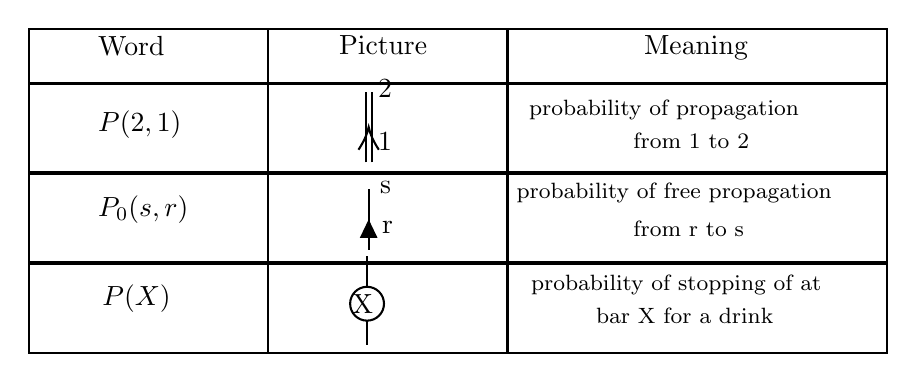
\begin{tikzpicture}[x=0.75pt,y=0.75pt,yscale=-1,xscale=1]
%uncomment if require: \path (0,349); %set diagram left start at 0, and has height of 349

%Shape: Rectangle [id:dp3972753239553969] 
\draw   (212.78,159.32) -- (328.11,159.32) -- (328.11,185.7) -- (212.78,185.7) -- cycle ;
%Shape: Rectangle [id:dp013530620031451002] 
\draw   (328.11,159.32) -- (443.44,159.32) -- (443.44,185.7) -- (328.11,185.7) -- cycle ;
%Shape: Rectangle [id:dp736076383888415] 
\draw   (443.44,159.32) -- (626.17,159.32) -- (626.17,185.7) -- (443.44,185.7) -- cycle ;
%Shape: Rectangle [id:dp018483080609867475] 
\draw   (212.78,185.32) -- (328.11,185.32) -- (328.11,229.2) -- (212.78,229.2) -- cycle ;
%Shape: Rectangle [id:dp18336509171990412] 
\draw   (328.11,185.32) -- (443.44,185.32) -- (443.44,229.2) -- (328.11,229.2) -- cycle ;
%Shape: Rectangle [id:dp5452879627568872] 
\draw   (443.44,185.32) -- (626.17,185.32) -- (626.17,229.2) -- (443.44,229.2) -- cycle ;
%Shape: Rectangle [id:dp710141061414926] 
\draw   (212.78,228.57) -- (328.11,228.57) -- (328.11,272.45) -- (212.78,272.45) -- cycle ;
%Shape: Rectangle [id:dp6981715844716105] 
\draw   (328.11,228.57) -- (443.44,228.57) -- (443.44,272.45) -- (328.11,272.45) -- cycle ;
%Shape: Rectangle [id:dp9707206740138988] 
\draw   (443.44,228.57) -- (626.17,228.57) -- (626.17,272.45) -- (443.44,272.45) -- cycle ;
%Shape: Rectangle [id:dp7188406169431831] 
\draw   (212.78,271.81) -- (328.11,271.81) -- (328.11,315.7) -- (212.78,315.7) -- cycle ;
%Shape: Rectangle [id:dp35373677352561617] 
\draw   (328.11,271.81) -- (443.44,271.81) -- (443.44,315.7) -- (328.11,315.7) -- cycle ;
%Shape: Rectangle [id:dp7761518007990666] 
\draw   (443.44,271.81) -- (626.17,271.81) -- (626.17,315.7) -- (443.44,315.7) -- cycle ;
%Straight Lines [id:da3953067075421305] 
\draw    (375.07,223.7) -- (375.07,189.7)(378.07,223.7) -- (378.07,189.7) ;
\draw [shift={(376.57,206.7)}, rotate = 450] [color={rgb, 255:red, 0; green, 0; blue, 0 }  ][line width=0.75]    (10.93,-4.9) .. controls (6.95,-2.3) and (3.31,-0.67) .. (0,0) .. controls (3.31,0.67) and (6.95,2.3) .. (10.93,4.9)   ;
%Straight Lines [id:da5701847229817978] 
\draw    (376.57,265.7) -- (376.57,236.7) ;
\draw [shift={(376.57,251.2)}, rotate = 450] [fill={rgb, 255:red, 0; green, 0; blue, 0 }  ][line width=0.08]  [draw opacity=0] (8.93,-4.29) -- (0,0) -- (8.93,4.29) -- cycle    ;
%Shape: Ellipse [id:dp16063069982491784] 
\draw   (367.64,291.82) .. controls (367.64,287.31) and (371.29,283.66) .. (375.79,283.66) .. controls (380.3,283.66) and (383.95,287.31) .. (383.95,291.82) .. controls (383.95,296.32) and (380.3,299.97) .. (375.79,299.97) .. controls (371.29,299.97) and (367.64,296.32) .. (367.64,291.82) -- cycle ;
%Straight Lines [id:da2549697012881261] 
\draw    (375.79,283.66) -- (375.79,268.7) ;
%Straight Lines [id:da05824951890975272] 
\draw    (375.79,311.7) -- (375.79,299.97) ;

% Text Node
\draw (244.78,161.32) node [anchor=north west][inner sep=0.75pt]   [align=left] {Word};
% Text Node
\draw (360.78,161.32) node [anchor=north west][inner sep=0.75pt]   [align=left] {Picture};
% Text Node
\draw (507.78,161.32) node [anchor=north west][inner sep=0.75pt]   [align=left] {Meaning};
% Text Node
\draw (244.78,197.32) node [anchor=north west][inner sep=0.75pt]    {$P( 2,1)$};
% Text Node
\draw (379.57,207.76) node [anchor=north west][inner sep=0.75pt]   [align=left] {1};
% Text Node
\draw (379.57,182.54) node [anchor=north west][inner sep=0.75pt]   [align=left] {2};
% Text Node
\draw (244.78,238.32) node [anchor=north west][inner sep=0.75pt]    {$P_{0}( s,r)$};
% Text Node
\draw (381.57,250.76) node [anchor=north west][inner sep=0.75pt]   [align=left] {r};
% Text Node
\draw (380.57,231.7) node [anchor=north west][inner sep=0.75pt]   [align=left] {s};
% Text Node
\draw (367.2,285.75) node [anchor=north west][inner sep=0.75pt]   [align=left] {X};
% Text Node
\draw (246.78,281.32) node [anchor=north west][inner sep=0.75pt]    {$P( X)$};
% Text Node
\draw (452.33,192.32) node [anchor=north west][inner sep=0.75pt]  [font=\footnotesize] [align=left] {probability of propagation };
% Text Node
\draw (502.63,208.32) node [anchor=north west][inner sep=0.75pt]  [font=\footnotesize] [align=left] {from 1 to 2};
% Text Node
\draw (446.33,232.32) node [anchor=north west][inner sep=0.75pt]  [font=\footnotesize] [align=left] {probability of free propagation };
% Text Node
\draw (502.63,250.32) node [anchor=north west][inner sep=0.75pt]  [font=\footnotesize] [align=left] {from r to s};
% Text Node
\draw (453.33,276.32) node [anchor=north west][inner sep=0.75pt]  [font=\footnotesize] [align=left] {probability of stopping of at \ };
% Text Node
\draw (484.63,292.32) node [anchor=north west][inner sep=0.75pt]  [font=\footnotesize] [align=left] {bar X for a drink};


\end{tikzpicture}

    \caption{Diagram dictionary for drunken man}
    \label{fig:drunken-man-1}
\end{figure}
The perturbation series in diagrams for this drunken man propagator is therefore
\begin{figure}[H]
    \centering
    


\tikzset{every picture/.style={line width=0.75pt}} %set default line width to 0.75pt        

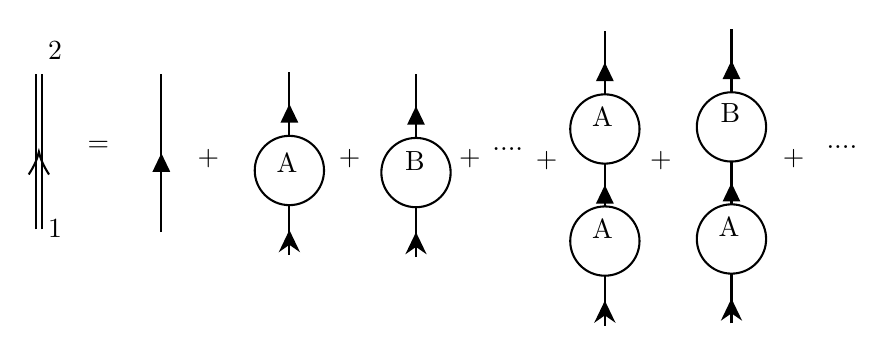
\begin{tikzpicture}[x=0.75pt,y=0.75pt,yscale=-1,xscale=1]
%uncomment if require: \path (0,349); %set diagram left start at 0, and has height of 349

%Straight Lines [id:da4757935872975344] 
\draw    (8.07,101.32) -- (8.07,26.7)(11.07,101.32) -- (11.07,26.7) ;
\draw [shift={(9.57,64.01)}, rotate = 450] [color={rgb, 255:red, 0; green, 0; blue, 0 }  ][line width=0.75]    (10.93,-4.9) .. controls (6.95,-2.3) and (3.31,-0.67) .. (0,0) .. controls (3.31,0.67) and (6.95,2.3) .. (10.93,4.9)   ;
%Straight Lines [id:da23622371172830803] 
\draw    (68.57,102.7) -- (68.57,26.7) ;
\draw [shift={(68.57,64.7)}, rotate = 450] [fill={rgb, 255:red, 0; green, 0; blue, 0 }  ][line width=0.08]  [draw opacity=0] (8.93,-4.29) -- (0,0) -- (8.93,4.29) -- cycle    ;
%Shape: Circle [id:dp4139523862436749] 
\draw   (113.57,73.01) .. controls (113.57,63.79) and (121.04,56.32) .. (130.26,56.32) .. controls (139.48,56.32) and (146.95,63.79) .. (146.95,73.01) .. controls (146.95,82.23) and (139.48,89.7) .. (130.26,89.7) .. controls (121.04,89.7) and (113.57,82.23) .. (113.57,73.01) -- cycle ;
%Straight Lines [id:da33169967910609544] 
\draw    (130.26,56.32) -- (130.26,25.7) ;
\draw [shift={(130.26,41.01)}, rotate = 450] [fill={rgb, 255:red, 0; green, 0; blue, 0 }  ][line width=0.08]  [draw opacity=0] (8.93,-4.29) -- (0,0) -- (8.93,4.29) -- cycle    ;
%Straight Lines [id:da28347419222198567] 
\draw    (130.26,113.7) -- (130.26,89.7) ;
\draw [shift={(130.26,101.7)}, rotate = 450] [fill={rgb, 255:red, 0; green, 0; blue, 0 }  ][line width=0.08]  [draw opacity=0] (10.72,-5.15) -- (0,0) -- (10.72,5.15) -- (7.12,0) -- cycle    ;
%Shape: Circle [id:dp1723289826034129] 
\draw   (174.57,74.01) .. controls (174.57,64.79) and (182.04,57.32) .. (191.26,57.32) .. controls (200.48,57.32) and (207.95,64.79) .. (207.95,74.01) .. controls (207.95,83.23) and (200.48,90.7) .. (191.26,90.7) .. controls (182.04,90.7) and (174.57,83.23) .. (174.57,74.01) -- cycle ;
%Straight Lines [id:da40381754331686626] 
\draw    (191.26,57.32) -- (191.26,26.7) ;
\draw [shift={(191.26,42.01)}, rotate = 450] [fill={rgb, 255:red, 0; green, 0; blue, 0 }  ][line width=0.08]  [draw opacity=0] (8.93,-4.29) -- (0,0) -- (8.93,4.29) -- cycle    ;
%Straight Lines [id:da5172106067784763] 
\draw    (191.26,114.7) -- (191.26,90.7) ;
\draw [shift={(191.26,102.7)}, rotate = 450] [fill={rgb, 255:red, 0; green, 0; blue, 0 }  ][line width=0.08]  [draw opacity=0] (10.72,-5.15) -- (0,0) -- (10.72,5.15) -- (7.12,0) -- cycle    ;
%Shape: Circle [id:dp663325870350397] 
\draw   (265.57,107.01) .. controls (265.57,97.79) and (273.04,90.32) .. (282.26,90.32) .. controls (291.48,90.32) and (298.95,97.79) .. (298.95,107.01) .. controls (298.95,116.23) and (291.48,123.7) .. (282.26,123.7) .. controls (273.04,123.7) and (265.57,116.23) .. (265.57,107.01) -- cycle ;
%Straight Lines [id:da6913773132395338] 
\draw    (282.26,36.32) -- (282.26,5.7) ;
\draw [shift={(282.26,21.01)}, rotate = 450] [fill={rgb, 255:red, 0; green, 0; blue, 0 }  ][line width=0.08]  [draw opacity=0] (8.93,-4.29) -- (0,0) -- (8.93,4.29) -- cycle    ;
%Straight Lines [id:da4724377841227787] 
\draw    (282.26,147.7) -- (282.26,123.7) ;
\draw [shift={(282.26,135.7)}, rotate = 450] [fill={rgb, 255:red, 0; green, 0; blue, 0 }  ][line width=0.08]  [draw opacity=0] (10.72,-5.15) -- (0,0) -- (10.72,5.15) -- (7.12,0) -- cycle    ;
%Shape: Circle [id:dp29262051024858293] 
\draw   (265.57,53.01) .. controls (265.57,43.79) and (273.04,36.32) .. (282.26,36.32) .. controls (291.48,36.32) and (298.95,43.79) .. (298.95,53.01) .. controls (298.95,62.23) and (291.48,69.7) .. (282.26,69.7) .. controls (273.04,69.7) and (265.57,62.23) .. (265.57,53.01) -- cycle ;
%Straight Lines [id:da2293551017015375] 
\draw    (282.26,69.7) -- (282.26,90.32) ;
\draw [shift={(282.26,80.01)}, rotate = 90] [fill={rgb, 255:red, 0; green, 0; blue, 0 }  ][line width=0.08]  [draw opacity=0] (8.93,-4.29) -- (0,0) -- (8.93,4.29) -- cycle    ;
%Shape: Circle [id:dp5742274191772756] 
\draw   (326.57,106.01) .. controls (326.57,96.79) and (334.04,89.32) .. (343.26,89.32) .. controls (352.48,89.32) and (359.95,96.79) .. (359.95,106.01) .. controls (359.95,115.23) and (352.48,122.7) .. (343.26,122.7) .. controls (334.04,122.7) and (326.57,115.23) .. (326.57,106.01) -- cycle ;
%Straight Lines [id:da8337372469854066] 
\draw    (343.26,35.32) -- (343.26,4.7) ;
\draw [shift={(343.26,20.01)}, rotate = 450] [fill={rgb, 255:red, 0; green, 0; blue, 0 }  ][line width=0.08]  [draw opacity=0] (8.93,-4.29) -- (0,0) -- (8.93,4.29) -- cycle    ;
%Straight Lines [id:da42712440571211296] 
\draw    (343.26,146.7) -- (343.26,122.7) ;
\draw [shift={(343.26,134.7)}, rotate = 450] [fill={rgb, 255:red, 0; green, 0; blue, 0 }  ][line width=0.08]  [draw opacity=0] (10.72,-5.15) -- (0,0) -- (10.72,5.15) -- (7.12,0) -- cycle    ;
%Shape: Circle [id:dp5287893719741432] 
\draw   (326.57,52.01) .. controls (326.57,42.79) and (334.04,35.32) .. (343.26,35.32) .. controls (352.48,35.32) and (359.95,42.79) .. (359.95,52.01) .. controls (359.95,61.23) and (352.48,68.7) .. (343.26,68.7) .. controls (334.04,68.7) and (326.57,61.23) .. (326.57,52.01) -- cycle ;
%Straight Lines [id:da8377025286119076] 
\draw    (343.26,68.7) -- (343.26,89.32) ;
\draw [shift={(343.26,79.01)}, rotate = 90] [fill={rgb, 255:red, 0; green, 0; blue, 0 }  ][line width=0.08]  [draw opacity=0] (8.93,-4.29) -- (0,0) -- (8.93,4.29) -- cycle    ;

% Text Node
\draw (12.57,95.32) node [anchor=north west][inner sep=0.75pt]   [align=left] {1};
% Text Node
\draw (12.57,9.32) node [anchor=north west][inner sep=0.75pt]   [align=left] {2};
% Text Node
\draw (31.57,57.32) node [anchor=north west][inner sep=0.75pt]   [align=left] {=};
% Text Node
\draw (122.57,63.32) node [anchor=north west][inner sep=0.75pt]   [align=left] {A};
% Text Node
\draw (184.57,62.32) node [anchor=north west][inner sep=0.75pt]   [align=left] {B};
% Text Node
\draw (336.57,39.32) node [anchor=north west][inner sep=0.75pt]   [align=left] {B};
% Text Node
\draw (335.57,94.32) node [anchor=north west][inner sep=0.75pt]   [align=left] {A};
% Text Node
\draw (274.57,95.32) node [anchor=north west][inner sep=0.75pt]   [align=left] {A};
% Text Node
\draw (274.57,41.32) node [anchor=north west][inner sep=0.75pt]   [align=left] {A};
% Text Node
\draw (84.57,61.32) node [anchor=north west][inner sep=0.75pt]    {$+$};
% Text Node
\draw (152.57,61.32) node [anchor=north west][inner sep=0.75pt]    {$+$};
% Text Node
\draw (210.57,61.32) node [anchor=north west][inner sep=0.75pt]    {$+$};
% Text Node
\draw (226.57,60.32) node [anchor=north west][inner sep=0.75pt]   [align=left] {....};
% Text Node
\draw (247.57,62.32) node [anchor=north west][inner sep=0.75pt]    {$+$};
% Text Node
\draw (302.57,62.32) node [anchor=north west][inner sep=0.75pt]    {$+$};
% Text Node
\draw (366.57,61.32) node [anchor=north west][inner sep=0.75pt]    {$+$};
% Text Node
\draw (387.57,59.32) node [anchor=north west][inner sep=0.75pt]   [align=left] {....};


\end{tikzpicture}

    \caption{Drunken man series}
    \label{fig:drunken-man-2}
\end{figure}

\subsection{Single-particle propagator for system of many interacting particles}

\subsection{The two-particle propagator and the particle-hole propagator}